% ******************************* Thesis Appendix B ********************************

\chapter{Desaf\'ios t\'ecnicos encontrados}

% **************************** Define Graphics Path **************************
\ifpdf
    \graphicspath{{Appendix2/Figs/Raster/}{Appendix2/Figs/PDF/}{Appendix2/Figs/}}
\else
    \graphicspath{{Appendix2/Figs/Vector/}{Appendix2/Figs/}}
\fi

Durante la ejecuci\'on del proyecto, nos enfrentamos a desaf\'ios y en particular de carácter t\'ecnico. Dentro de estos desaf\'ios podemos encontrar algunos que se destacan por su complejidad y dificultad para resolverlos y otros que se destacan por su severidad como riesgo tecnol\'ogico dentro del proyecto. Por ello consideramos apropiado incluir un ap\'endice en donde se hace menci\'on a los mismos y a sus respectivas soluciones.

\section{Problemas con SFPs y Patchcoords}

Los transceivers SFP+ son una componente de hardware utilizada en cada puerto f\'isico de la tarjeta NetFPGA en la construcci\'on del dispositivo RAU-Switch. Básicamente se encargan de implementar el mecanismo de acceso a la capa f\'isica, en este caso fibra \'optica.

Pueden encontrarse transceivers compatibles con patch cords de fibra \'optica monomodo, multimodo y compatibles con ambos tipos.

En el desarrollo de este proyecto se trabaj\'o con transceivers SFP+ compatibles con ambos tipos de patch cords, aunque para la construcci\'on de la red prototipo por razones econ\'omicas se utilizaron transceivers SFP+ compatibles solamente con patch cords de fibra multimodo.

\section{Desprogramaci\'on del hardware NetFPGA}
\label{apendiceB2}

En el desarrollo de este proyecto se utilizan dos estrategias diferentes para programar el hardware NetFPGA. La primera estrategia, detallada en la guía de ejecución del Test de Producción\citep{ProdTestManual}, permite de forma sencilla programar el hardware utilizando la herramienta Impact de la suite Xilinx ISE SDK. Sin embargo este procedimiento no persiste la programaci\'on del hardware, por lo que al producirse un corte de corriente en el circuito (apagado de la PC por ejemplo) el mismo pierde la programaci\'on. Este efecto puede comprobarse fácilmente utilizando la herramienta Impact para leer el valor de diferentes registros del hardware, los cuales indican el estado del mismo.

La segunda estrategia es la programación PCIe denominada en este trabajo como programación persistente, la cual utiliza la herramienta \textbf{pcieprog} de la plataforma NetFPGA para almacenar la programaci\'on del hardware en una de las unidades de memoria Flash del equipo. Concretamente este procedimiento implica programar el hardware con un proyecto compatible con la programaci\'on PCIe (es necesario que el proyecto implemente un m\'odulo para la configuraci\'on del chip FPGA desde una de las memorias Flash) utilizando la herramienta Impact. Luego se almacena en una de las unidades de memoria Flash un archivo binario con la implementaci\'on del proyecto con el cual se quiere programar el hardware. Luego al momento del encendido del equipo, el chip FPGA es programado desde el contenido almacenado en una de las memorias Flash.

De esta forma la programaci\'on del equipo se almacena de forma persistente, perdurando incluso cuando el equipo es apagado.

\section{Falta de licencias para suite de Xilinx ISE SDK}
\label{apendiceB3}
La suite de desarrollo Xilinx ISE SDK se compone por un conjunto extenso de herramientas para la progrmaci\'on y desarrollo de software utilizando los productos de este fabricante; entre los cuales se encuentra el chip Virtex 5 utilizado en el hardware NetFPGA. Estas herramientas de software son licenciadas lo que significa que para su uso es necesario contar con una licencia de software apropiada.

Cada herramienta particular de la suite Xilinx tiene una licencia particular y se agrupan en diferentes paquetes de licencias. De esta forma dependiendo del uso que se vaya a hacer de esta plataforma, el o los paquetes de licencias que se deben adquirir. Adem\'as cada licencia se corresponde con una herramienta para una familia de chips en particular. Por ejemplo para trabajar con las tarjetas NetFPGA-10G se necesitan licencias para el chip Virtex5 TX240T.

Xilinx ofrece un paquete de licencias gratuitas para trabajar con un conjunto reducido de herramientas (entre ellas se incluye el programa Impact) y un paquete de licencias completo de prueba por un tiempo de 30 d\'ias compatible con los \'ultimos modelos de chips (Virtex6 y Virtex7). Como dentro de estos paquetes no se incluyen las licencias necesarias para la programaci\'on PCIe (programaci\'on persistente) una alternativa es adquirir un paquete de licencias con un valor aproximado de USD500 por PC (costo en dolares americanos al mes de Setiembre del año 2014).

En este proyecto, por razones econ\'omicas primero se solicit\'o mediante el programa de soporte a Universidades de Xilinx el paquete de licencias necesario, a la vez que se inici\'o un contacto con el Instituto de Ingeniería Eléctrica de la Facultad de Ingeniería (IIE) solicitando orientación en relación a este problema. Finalmente se recibi\'o a través de dicho programa de apoyo a universidades una interesante donación de licencias, posibilitando una real explotación del hardware y la plataforma en su conjunto, aunque esta espera represent\'o un contratiempo en el cronograma inicial del proyecto. 

\section{Falta de driver para cable JTAG Xilinx}
Para la programación del hardware NetFPGA se utiliza un cable programador especial con una interfaz de conexi\'on JTAG.  Este cable presenta el inconveniente de que sus fabricantes no desarrollaron drivers para la distribución de Linux con la que se trabaja en este proyecto, existiendo drivers oficiales para entornos Windows y una versi\'on no oficial para la distribución Fedora.

Si bien inicialmente esto oblig\'o a programar el hardware en un ambiente Windows para realizar las pruebas de verificaci\'on del mismo (Producction Test y RLDRAM Test) finalmente se consigue un driver no oficial\cite{JtagD} tambi\'en compatible con Ubuntu 12.04, habilitando de esta forma a programar el hardware en la misma PC.

\section{Problemas t\'ecnicos con Open vSwitch}
\label{apendiceB5}

Open vSwitch es uno de los pilares fundamentales de RAU-Switch puesto que es el encargado de implementar el plano de datos de OpenFlow. Durante el desarrollo de este proyecto, en el tiempo empleado a la experimentaci\'on con esta herramienta, se genera conocimiento en relaci\'on a aspectos importantes sobre la herramienta; los cuales no son triviales y vale la pena mencionar en este apartado. A continuaci\'on se enumeran los siguientes:

\begin{enumerate}
\item Parte de las funcionalidades de Open vSwitch, est\'an implementadas en modo kernel y otra parte en modo usuario. Estas \'ultimas presentan un nivel de performance muy pobre en comparaci\'on a las primeras; y en particular las funcionalidades de MPLS se encuentran solamente disponibles en modo usuario.

\item De acuerdo a la p\'agina de preguntas frecuentes, la \'ultima versi\'on de Open vSwitch al momento de realizarse este proyecto, garantiza soporte a las operaciones de MATCH, PUSH y POP de hasta tres etiquetas MPLS apiladas, as\'i como su posterior procesamiento acorde al pipe de OpenFlow. Todas estas funcionalidades adem\'as se implementan en modo usuario.

Por otro lado, de acuerdo  a las notas de liberaci\'on de la versi\'on 2.3.1, solamente se garantiza el soporte a las funciones de MATCH, PUSH y POP de MPLS para un \'unico nivel de etiquetas; esto es una sola etiqueta MPLS. Luego se garantiza adem\'as el posterior procesamiento acorde al pipe OpenFlow. Esta informaci\'on no s\'olo es contradictoria, sino que adem\'as no se condice con la realidad. Experimentalmente se prueba que si bien la versi\'on 2.3.1 implementa correctamente las operaciones de MATCH y PUSH de una \'unica etiqueta MPLS, la operaci\'on POP no se encuentra implementada para esta versi\'on, rompiendo adem\'as el pipe de procesamiento OpenFlow. 

Afortunadamente \'este comportamiento hab\'ia sido detectado y reportado por otros usuarios de Open vSwitch como un BUG, resolviéndose posteriormente en la versi\'on de desarrollo \citep{OVSSourceCode}.

\item Trabajando con la versi\'on de desarrollo en el repositorio de c\'odigo fuente de Open vSwitch~\citep{OVSSourceCode} (rama master en el repositorio Git), se comprueba experimentalmente el soporte para las operaciones de Match, Push y Pop de hasta 3 etiquetas, as\'i como el posterior procesamiento del paquete seg\'un el pipe de  OpenFlow.

\item Puertos OpenFlow con direcciones IP:
 
Para lograr que cada interfaz f\'isica de la tarjeta NetFPGA se comporte tanto como un puerto OpenFlow, como una interfaz IP, es necesario:

\begin{enumerate}
\item Crear un bridge con Open vSwitch y agregar cada interaz f\'isica como un puerto OpenFlow al mismo.
\item Asignar una dirección IP a la propia intefaz f\'isica (por ejemplo utilizando el comando ifconfig).
\end{enumerate}

El comportamiento deseado por una interfaz h\'ibrida IP/OpenFlow en el prototipo ser\'ia el que se muestra en la figura ~\ref{fig:OVSInterfaces} (mitad izquierda). El paquete ingresa al router atrav\'es de la interfaz f\'isica \textbf{nf0} y de ah\'i en m\'as el procesamiento del mismo es delegado al m\'odulo de Open vSwitch en el kernel de Linux. Aqu\'i el paquete es procesado y tratado en consecuencia a lo que indica la tabla de flujos en Open vSwitch. En el prototipo, para este paquete existen dos alternativas: (1) se procesa el contenido del mismo y se reenv\'ia por otra interfaz acorde a la regla correspondiente, (2) es contemplado por una regla con la acci\'on \textit{NORMAL} y por tanto es procesado como lo har\'ia un switch legado (en este caso como lo procesar\'ia el kernel de linux).

\begin{figure}[h!] 
\centering    
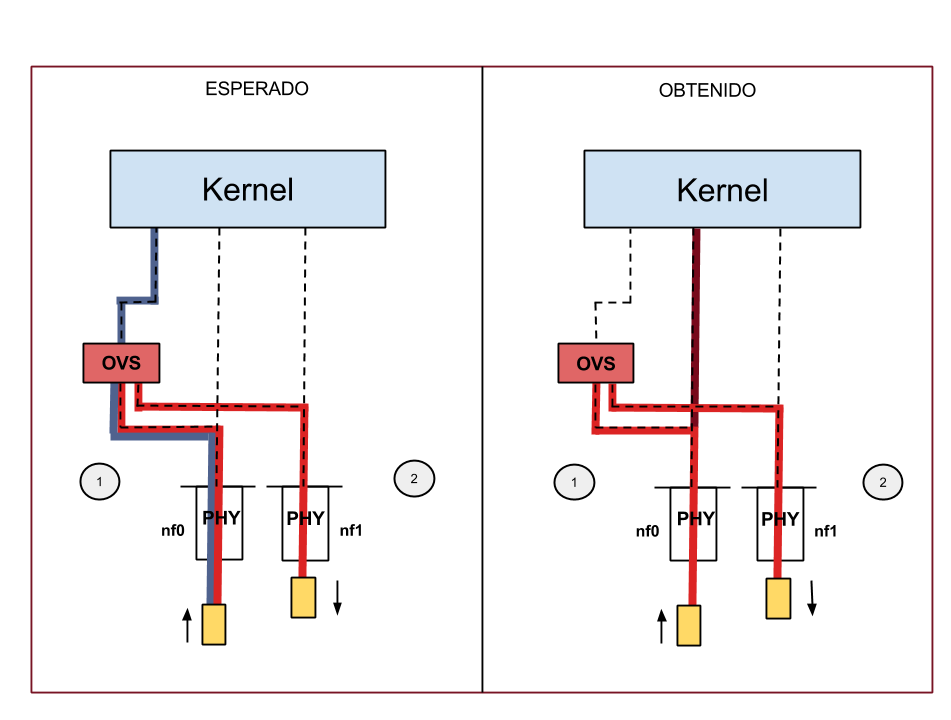
\includegraphics[width=0.65\textwidth]{ovs_figure3}
\caption[Funcionamiento de puertos Open vSwitch]{Funcionamiento de puertos Open vSwitch}
\label{fig:OVSInterfaces}
\end{figure}

No obstante, el procesamiento del paquete al ingresar por la interfaz f\'isica \textbf{nf0} difiere del comportamiento deseado (ver mitad derecha de la imagen). El paquete es procesado por Open vSwitch como se describi\'o anteriormente, pero tambi\'en es enviado para su procesamiento en el kernel de Linux.

Esto implica que el switch se comporte como una mezcla de un switch OpenFlow  con una PC Linux normal, ocasionando un tratamiento de paquetes en el prototipo diferente al especificado por las reglas OpenFlow calculadas.

Para solucionar este problema se utilizan interfaces virtuales de la siguiente forma:

\begin{enumerate}
\item Se crea una interfaz virtual por cada interfaz física y se conecta a través de dichas interfaces,  openvswitch con el kernel.

\item La dirección IP que antes se asignaba a cada interfaz física ahora se le asigna a su correspondiente interfaz virtual.

\item Se deja la interfaz física sin dirección IP y de esta forma se asegura que ningún paquete que arribe a dicha interfaz será procesado por el kernel, ya que nunca coincidirá la dirección IP que contenga un paquete con la dirección de la interfaz.

\item Se crean entradas de prioridad mínima en la tabla de flujos de openvswitch que indiquen que todo lo que entre por la interfaz física se envíe a través su correspondiente interfaz virtual y viceversa.

\item De esta forma si no hay un flujo de mayor prioridad para procesar los paquetes que entran por determinada interfaz física, estos serán enviados al kernel mediante la interfaz virtual, procesados por este para luego ser enviado por la interfaz virtual a la física y seguir su camino.

\item Estos pasos aseguran que todo el tráfico sea procesado por las tablas de Open vSwitch, y serán procesados por el kernel solo en caso de ser necesario.
\end{enumerate}

\begin{figure}[h!] 
\centering    
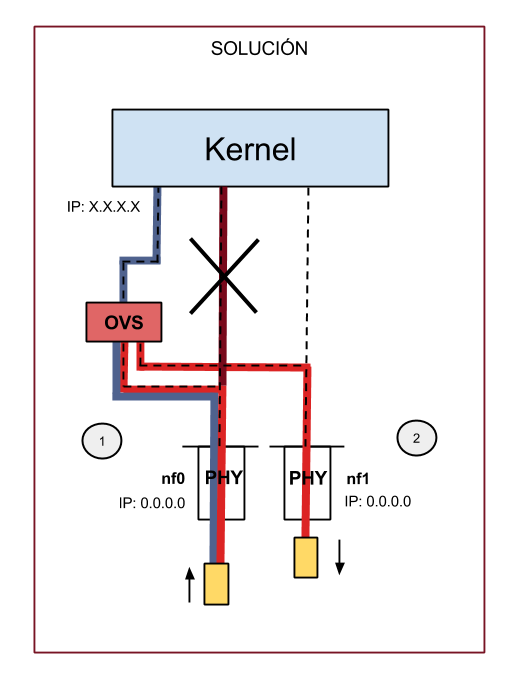
\includegraphics[width=0.35\textwidth]{ovs_figure4}
\caption[Puertos Open vSwitch - Soluci\'on propuesta]{Puertos Open vSwitch - Soluci\'on propuesta}
\label{fig:OVSInterfaces2}
\end{figure}

\end{enumerate}

\section{MPLS Linux y Quagga LDP}
\label{apendiceB6}

MPLS Linux es un proyecto orientado a dotar de funcionalidades de MPLS al Kernel de Linux, mediante un parche con el cual se extiende al mismo y el cual tras recompilarse queda pronto para brindar soporte nativo al protocolo MPLS.

Existen principalmente dos versiones: el proyecto original\cite{MplsLinux1} encabezado por James R. Leu el cual data de hace m\'as de 15 a\~nos y no cuenta con contribuciones importantes desde hace aproximadamente 9 y otro proyecto\cite{MplsLinux2} encabezado por Igor Maravick (quien trabaj\'o en el proyecto anterior) que data del a\~no 2010 y surge como una actualizaci\'on del proyecto original.

El primer proyecto fue pensado como un parche para el kernel de Linux versi\'on 2.6.3.16 (tener en cuenta que la versi\'on actual es la 4.1.1). Adicionalmente se desarroll\'o una extensión de la suite Quagga\cite{QuaggaLDP1} que implementa el algoritmo LDP para la construcci\'on de redes IP/MPLS.

Por otro lado, el proyecto de Igor Maravick es un kernel de Linux versi\'on 3.9.0-rc3 con las modificaciones necesarias para soportar el protocolo MPLS ya incorporadas. Adicionalmente existe una nueva extension de la suite Quagga que implementa el protocolo LDP \cite{QuaggaLDP2} y es compatible con esta versi\'on de MPLS-Linux.

En el contexto de este proyecto se trabaj\'o con ambas versiones de MPLS-Linux y las respectivas versiones de Quagga-LDP. Para la versi\'on original de MPLS-Linux se prob\'o compilar el parche con diferentes versiones de kernel, entre ellas las versiones 2.6.32.16 y 2.6.32.65 no pudiendo as\'i configurar correctamente el ambiente de trabajo. En particular estas versiones son tan antiguas que gran parte de las herramientas utilizadas para la construcci\'on de RAU-Switch no son compatibles. Adicionalmente se prueba compilar el parche para la versi\'on de kernel 3.11.0-15 generic (versi\'on que trae Ubuntu 12.01) pero tampoco se obtienen buenos resultados.

En relaci\'on a la versi\'on de Igor Maravik se logr\'o configurarla correctamente, as\'i como la extensi\'on Quagga-LDP. No obstante al momento de ejecutar dichas herramientas se detectaron problemas en la interacci\'on entre las mismas; mediante los logs de la herramienta Quagga se detectaron errores al momento de insertar entradas en las tablas MPLS del kernel.

Finalmente por la falta de información en relación a estas componentes, ya que sobre el proyecto original existe muy poca documentaci\'on mientras que para el proyecto de Igor Maravik no existe la misma, se decidi\'o descartar esta alternativa para implementar el algoritmo LDP. 